\section{An Overview of \Cogent}{\label{sec:cogent}}

\Cogent~\citep{OConnor:2016, OConnor:thesis, Cogent_JFP_2021} is a higher-order, polymorphic, purely functional programming
language, in the tradition of the pure subsets of languages such as
Haskell or ML. Programs are expressed as mathematical functions
operating on algebraic data types. Unlike Haskell or ML, however,
\Cogent is designed for implementing low-level systems code where manual
memory management is essential for performance reasons. As such,
\Cogent has no garbage collection mechanism and heap (de)allocations are
explicit in the language.

The \cogent language is equipped with a \emph{uniqueness type
system}~\citep{wadler:90, clean:93}, enabling a seamless transition from a
purely functional semantics to an imperative semantics and a compilation
strategy to generate efficient low-level C code.
%
The certifying compiler automatically produces a formal
proof~\citep{Rizkallah:itp16} that its generated C code refines an Isabelle/HOL
embedding of the \cogent program's functional semantics. \Cogent was used to
implement two real-world file systems and to verify the correctness of key file
system operations~\citep{Amani:2016}.
%The \cogent language and its verification were introduced
%by~\citepos{OConnor:2016,} and most recently presented by
%\citeauthor{OConnor:thesis} in his PhD
%thesis~\cite{OConnor:thesis}. Real-world applications using \cogent for
%certifying file systems are presented by~\citepos{Amani:2016} (see also
%\citepos['s PhD thesis]{Amani:phd}). 
This section summarises aspects of \cogent and its verification framework that
are relevant to our work.

\subsection{\Cogent's Uniqueness Types System}

Uniqueness type systems ensure that each \emph{linear} object in memory
is uniquely referenced. Consequently, updates to these objects in a
purely functional language can be compiled as in-place destructive
updates, without the need for copying~\citep{wadler:90}. In \cogent, we
call the type of objects that are subject to the uniqueness restrictions
\emph{linear types}, and the rest \emph{non-linear types}.  Roughly
speaking, any object that resides in the heap or contains pointers to
other heap-objects --- and is not \emph{read-only} (explained later) ---
is linear; otherwise it is non-linear.  In the generated C code, all
pointers address heap memory.  This is because \cogent's verification
framework depends on the AutoCorres library~\citep{autocorres}, which
does not support stack pointers.  Therefore, we can summarise the
linearity of an object simply as: A linear object is behind a pointer
and/or contains pointers.
%% Later we will see that the linearity of a type is closely correlated
%% to the \dargent layouts.

As a simple \cogent example, consider the following code.
\begin{lstlisting}[language=Cogent]
  type Bag = { count : U32, sum : U32 }
  
  addToBag : (U32, Bag) -> Bag
  addToBag (x, bag {count = c, sum = s}) = bag {count = c + 1 , sum = s + x }
\end{lstlisting}
The first line declares a linear record type \cg|Bag|, which is a record
comprised of two 32-bit unsigned words. In the \cg|addToBag| function,
we retrieve the value of the two fields by pattern matching and 
update both fields of the record according to the given input.
It is compiled to a C function that takes as input a pointer to a bag
structure and updates it \emph{in place}, because the uniqueness type 
system ensures that the \cg|Bag| object is uniquely referenced.


\begin{figure}
\[
\begin{array}{llclr}
  \text{Types} 
     & \tau & ::=  & T & \text{(primitive types)} \\
     &      & \mid & ()                & \text{(unit)} \\
     &      & \mid & \alpha            & \text{(type variables)} \\
     % &      & \mid & \tau_1 \rightarrow \tau_2      & \text{(functions)} \\
     &      & \mid &\RecordTy{\many{\mathrm{f}_i : \tau_i}}{s} & \text{(records)}\\
     &      & \mid & \VariantTy{\many{\mathrm{A}_i\ \tau_i}}  & \text{{(variants)}}\\
     &      & \mid & \AbsTy{K}{\many{{\tau_i}}}{s}  & \text{(abstract types)} \\
     &      & \mid & \dots & \\
  \text{Primitive types} & T & ::= & \PrimType{U}n \mid \PrimType{Bool} & \text{($n = 1 \dots 64$)} \\
  \text{Field names}  & & \ni  & \mathrm{f}\\
  \text{Constructors} & & \ni  & \mathrm{A}\\
  \text{Sigils} & s & ::= & \BoxedNL \mid \Unboxed & \\
                & \BoxedNL & ::= & \ModeN{w} \mid \ModeN{r} & 
\end{array}
\]
(lists are represented by $\many{\text{overlines}}$)
\caption{The syntax of \cogent types}
\label{fig:syntax-cogent-types}
\end{figure}


The syntax of (a relevant subset of) \cogent's types is given in \autoref{fig:syntax-cogent-types}.
\cogent \emph{primitive} types include the $n$-bit unsigned integer
types, $\PrimType{U}n$ (where $n = 1 \dots 64$), and booleans ($\PrimType{Bool}$).
Among the $\PrimType{U}n$ types, we call them \emph{word-sized integers} (or simply
\emph{words}) when $n \in \{8,16,32,64\}$. Algebraic data types can be formed using
\emph{record} and \emph{variant} types (aka.\ tagged unions).
%
Furthermore, \cogent supports declaring \emph{abstract types} with their
definitions provided in C.
%
\cogent employs a structural type system, meaning that compound types, as well as their subtyping
relations, are defined solely by their structure and the structure of their components. Names given to types such as $\mathtt{Bag}$ above are type synonyms---mere abbreviations for better cosmetics. 


\cogent's type system distinguishes between \emph{boxed} and
\emph{unboxed} types through a \emph{sigil} annotation on the type.
The boxedness of a type characterises how an object is referenced---by-value or by-pointer.
An object of a boxed type (sigil $\BoxedNL$) is accessed via its pointer.
Because in \cogent, all pointers address heap memory, a boxed object must reside in the heap.
An object of an unboxed type (sigil $\Unboxed$) is accessed by value and either
resides in the stack or is embedded inside a larger data structure in the
heap. In the latter case, when the object is accessed, it will be copied
by-value to a stack variable. The sigil is only used in the \cogent core calculus.
For example, the type \cg{Bag} we showed earlier is desugared to $\RecordTy{
  \FieldTy{count}{\PrimType{U32}}, \FieldTy{sum}{\PrimType{U32}}}{\BoxedNL}$, as it is 
a boxed record.

The uniqueness and the boxedness of a type are concerned with different
aspects of memory locations.  The uniqueness relates to \emph{what} kind
of memory the object references (linear or non-linear), whereas the
boxedness of an object determines \emph{how} its memory is referenced
(by-value or by-pointer).
%
Since all pointers in \cogent point to the heap, any boxed object must
be linear (with the same caveat that it must not be read-only) because
it is directly behind a pointer. The converse is not true though. A
typical counter-example is a stack-allocated structure that contains
pointers; this structure is linear but unboxed.

Records and abstract types can be either boxed or unboxed. Primitive types and
variant types, however, can only be unboxed. For this reason, primitives and
variants do not include a sigil. For a boxed type, \cogent allows further
fine-grained control of accessibility: A boxed type can either be writable
(with sigil $\ModeN{w}$) or read-only (with sigil $\ModeN{r}$). When a type
has a read-only sigil, even though it is behind a pointer or contains pointers,
it becomes non-linear---this is the caveat we mentioned earlier in this section.
This read-only object can be shared analogously to how a variable can be immutably borrowed
in the type system of Rust~\citep[\S~4.2]{rust-borrow}.

Before \dargent{}, the \cogent compiler used a pre-defined code generation algorithm to compile
data types to C.
A record type in \cogent was mapped to a C
struct, with the fields laid out in the order in which they are declared in the
type. The mapping for variant types, on the other hand, was less direct:
\Cogent's verification tool chain does not support C unions, so variants were also represented as structs in C, containing a field for a tag, and a field for each alternative's payload.

Applying such a fixed code generation scheme is no surprise for a typical high-level
functional language,
whose implementation details are hidden from the language users. But \cogent is not just a functional language, it is also a systems language where
the exact low-level representation of data types is relevant to programmers.
This fixed code generation algorithm often resulted in
suboptimal or undesired representations of \cogent types in C, and users of the 
\cogent language had to know
about the implementation details of the code generator in order to write
C code that directly interfaces with \cogent programs. In situations where
the \cogent program needs to interoperate with existing C components, say,
when developing an operating system component that interfaces with the Linux
kernel headers, glue code was required to translate between representations, resulting in development
and run-time overhead. \liam{Perhaps we should add some Bilby numbers here}
%
%% CMCL: Reword sentence below
%%
Also, problematically, as this glue code depended on the representation choices
made by the \cogent compiler, future versions of the compiler could break
previously working code due to changes in the code generation scheme.

\subsection{The Verification Framework}
{\label{ssec:cogent-verification}}

In addition to a programming language, \Cogent is also a verification framework
realised in Isabelle/HOL, based on \emph{certifying compilation}.
Compiling a \cogent program results in multiple components:
\begin{enumerate}
  \item a C program,
  \item an Isabelle/HOL \emph{shallow embedding}   of the \cogent program,
  \item an Isabelle/HOL \emph{deep embedding}   of the \cogent program,
  \item an Isabelle proof of refinement between the C
      program and the Isabelle shallow embedding.
\end{enumerate}
The last item relies on the AutoCorres library~\citep{autocorres} to generate 
a representation of the C code in Isabelle/HOL. More precisely, the AutoCorres library 
abstracts the C semantics via a SIMPL~\citep{simpl} formal language into
a monadic embedding in Isabelle/HOL.

This compilation process provides an indirect way of formally verifying
properties about the generated C program. The user first proves
the desired properties about the Isabelle shallow
embedding.  This manual proof should follow by simple equational reasoning about HOL terms by applying term rewriting
tactics provided by the theorem prover. Then, the automatic refinement
proof between the C code and the shallow embedding transports the proven
properties to the C program. In short, \cogent's verification
framework reduces complicated low-level verification on the C program to
a simple high-level equational proof.

The compiler-generated refinement proof between the C code and the
Isabelle shallow embedding is composed of several smaller
correspondence proofs.  When the compiler generates the shallow
embedding of the \cogent program in Isabelle, it also generates a
\emph{deep embedding} representing the abstract syntax of the \cogent
program. Two semantics are assigned to the deep embedding: a purely
functional \emph{value semantics}, and a stateful \emph{update
  semantics}, with pointers, memory states, and in-place field updating.
It is proved once-and-for-all that these two semantics are equivalent for
any well-typed \cogent program. As part of the certifying compilation,
the compiler produces a refinement proof between the shallow embedding
and the deep embedding with value semantics, and a refinement proof
between the deep embedding with update semantics and the monadic C
embedding obtained from AutoCorres. Chaining the three correspondence
lemmas results in a correspondence between
the shallow embedding and the C program, stating that the C program is a
refinement of the \cogent program's semantics (see \autoref{fig:cogent_framework}).

\begin{figure}
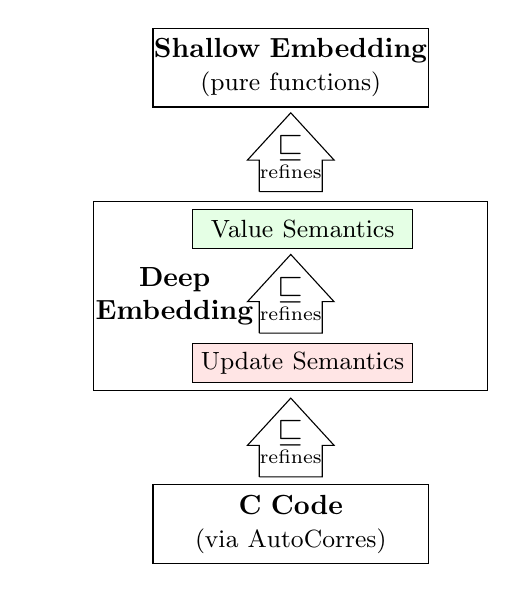
\begin{tikzpicture}
  \draw (0,0.5) rectangle (3.5,1.5) node[pos=0.5, text width=3.5cm, align=center] 
        {\textbf{Shallow Embedding} \\ \small (pure functions)};
  \draw (-0.75,-0.7) rectangle (4.25,-3.1) node[xshift=0.4cm, pos=0.5, text width=3.5cm, align=center, anchor=east] 
        {\textbf{Deep\\Embedding}};
  \draw [fill=green!10] (0.5,-0.8) rectangle (3.3,-1.3) node[pos=0.5, text width=3.5cm, align=center] 
        {{\small Value Semantics}};
  \begin{scope}[yshift=2cm - 3.5pt]
    \draw  (1.35,-4.25) -- (1.35,-3.85) -- (1.2,-3.85) -- (1.75,-3.25) -- (2.3,-3.85) -- (2.15,-3.85)
           -- (2.15,-4.25) -- (1.35,-4.25);
    \node [text width=1cm, align=center] at (1.74,-3.7) {\large ${\sqsubseteq}$};
    \node [text width=1cm, align=center] at (1.75,-4) {\scriptsize refines};
  \end{scope}

  \draw [fill=red!10] (0.5,-2.5) rectangle (3.3,-3) node[pos=0.5, text width=3.5cm, align=center] 
        {{\small Update Semantics}};
  \draw (0,-5.3) rectangle (3.5,-4.3) node[pos=0.5, text width=3.5cm, align=center] 
        {\textbf{C Code} \\ \small (via AutoCorres)};
  \begin{scope}[xshift=0,yshift=5pt]
    \draw  (1.35,-0.75) -- (1.35,-0.35) -- (1.2,-0.35) -- (1.75,0.25) -- (2.3,-0.35) -- (2.15,-0.35)
           -- (2.15,-0.75) -- (1.35,-0.75);
    \node [text width=1cm, align=center] at (1.74,-0.2) {\large ${\sqsubseteq}$};
    \node [text width=1cm, align=center] at (1.75,-0.5) {\scriptsize refines};
  \end{scope}
  \begin{scope}[yshift=1.5pt]
    \draw  (1.35,-4.25) -- (1.35,-3.85) -- (1.2,-3.85) -- (1.75,-3.25) -- (2.3,-3.85) -- (2.15,-3.85)
           -- (2.15,-4.25) -- (1.35,-4.25);
    \node [text width=1cm, align=center] at (1.74,-3.7) {\large ${\sqsubseteq}$};
    \node [text width=1cm, align=center] at (1.75,-4) {\scriptsize refines};
  \end{scope}
\end{tikzpicture}

\caption{The \cogent refinement framework.}
\label{fig:cogent_framework}
\end{figure}

